\documentclass[a4paper]{article}

\usepackage{color}
\usepackage{url}
\usepackage[T2A]{fontenc} 
\usepackage[utf8]{inputenc}
\usepackage{graphicx}

\usepackage[english,serbian]{babel}

\begin{document}

\section{Slučaj upotrebe: Pregled dana i unetih radnih sati za odredjeni mesec}
\begin{enumerate}
    \item \textbf{Kratak opis:} Zaposleni na osnovu odabira meseca pregleda radne dane, unete sate i kratke opise poslova.
    \item \textbf{Učesnici:}
        \begin{itemize}
            \item Zaposleni
        \end{itemize}
    \item \textbf{Preduslovi:} Zaposleni je registrovani korisnik sistema.
    \item \textbf{Postuslovi:} Zaposlenom je prikazana lista tiketa za odabrani mesec, gde je za svaki tiket prikazan dan, broj sati odrađenih za taj dan i kratak opis posla odrađenog za taj dan.
    \item \textbf{Osnovni tok:}
        \begin{enumerate}
            \item Zaposleni otvara stranicu za unošenje radnih sati.
            \item U padajućoj listi zaposleni bira za koji mesec želi da mu se prikažu uneti dani sa odgovarajućim podacima.
            \item Sistem vrši obradu zahteva.
            \item Na stranici se prikazuje lista tiketa, gde svaki tiket sadrži podatke o unetom danu, broju radnih sati za taj dan i opisu odradjenog posla.
        \end{enumerate}
    \item \textbf{Alternativni tokovi:} 
        \begin{enumerate}
            \item \textbf{Zaposleni je odabrao tekući mesec u padajućoj listi}. Ukoliko u koraku (b) zaposleni odabere tekući mesec, zaposlenom se nakon završetka procesa (d) prikazuje dugme sa opcijom dodavanja novog tiketa.
        \end{enumerate}
    \item \textbf{Podtokovi:} /
    \item \textbf{Specijalni zahtevi:} /
    \item \textbf{Dodatne informacije:} /
\end{enumerate}



\section{Slučaj upotrebe: Unošenje radnih sati}
\begin{enumerate}
    \item \textbf{Kratak opis:} Zaposleni unosi broj odrađenih ranih sati za konkretan dan kao i opis odrađenog posla.
    \item \textbf{Učesnici:}
        \begin{itemize}
            \item Zaposleni
        \end{itemize}
    \item \textbf{Preduslovi:} Zaposleni je registrovani korisnik sistema i na stranici za pregled radnih sati je odabrao tekući mesec.
    \item \textbf{Postuslovi:} Odrađen broj radnih sati za konkretan dan je sačuvan u sistemu. Baza je ažurirana. Na stranici se prikazuje novi tiket koji je u nerazrešenom statusu.
    \item \textbf{Osnovni tok:}
        \begin{enumerate}
            \item Zaposleni pritiska dugme za dodavanje novog tiketa.
            \item Prikazuje se forma koji sadrži polja za odabir dana, broj odrađenih radnih sati, i opis odrađenog posla.
            \item Zaposleni popunjava formu.
            \item Potvrđuje unos za taj dan.
            \item Sistem vrši obradu podataka.
            \item Sistem čuva unete podatke u bazi podataka.
            \item Na stranici se dodaje tiket koji je u nerazrešenom statusu i informacije koje je korisnik uneo za taj dan.
        \end{enumerate}
    \item \textbf{Alternativni tokovi:}
        \begin{enumerate}
            \item \textbf{Zaposleni je odabrao nevalidan dan}. Ukoliko u koraku (d) korisnik potvrdi unos za dan za koji je uneo radne sate ili dan koji je ispred trenutnog dana ili unese negativan broj za radne sate, prikazuje mu se odgovarajuća poruka o grešci. Proces se nastavlja u koraku (c).
        \end{enumerate}
    \item \textbf{Podtokovi:} /
    \item \textbf{Specijalni zahtevi:} /
    \item \textbf{Dodatne informacije:} Polje za unošenje broja radnih sati je obavezno.
\end{enumerate}


\includegraphics[scale=0.5]{PrijavljivanjeRadnogVremena.jpg}





\section{Slučaj upotrebe: Izmena tiketa}
\begin{enumerate}
    \item \textbf{Kratak opis:} Zaposleni menja informacije u tiketu za konkretan dan.
    \item \textbf{Učesnici:}
        \begin{itemize}
            \item Zaposleni
        \end{itemize}
    \item \textbf{Preduslovi:} Zaposleni je registrovani korisnik sistema, na stranici za pregled radnih sati je odabrao tekući mesec i tiket za dan čije informacije korisnik želi da menja je prikazan na stranici, postoji u sistemu i u nerazrešenom je statusu.
    \item \textbf{Postuslovi:} Informacije su ažurirane u sistemu i korisnik vidi promene na tiketu .
    \item \textbf{Osnovni tok:}
        \begin{enumerate}
            \item Zaposleni pritiska odgovarajuće dugme za izmenu podataka na tiketu.
            \item Na tiketu polja za unošenje radnih sati i opis odrađenog posla postaju moguća za izmenu.
            \item Zaposleni menja odgovarajuća polja.
            \item Potvrđuje izmene.
            \item Sistem vrši obradu podataka.
            \item Sistem čuva unete podatke u bazi podataka.
            \item Na stranici se prikazuje tiket u izmenjenom obliku.
        \end{enumerate}
    \item \textbf{Alternativni tokovi:}
        \begin{enumerate}
            \item \textbf{Zaposleni je odabrao nevalidan broj radnih sati}. Ukoliko u koraku (c) zaposleni unese radne sate koji predstavljaju negativan broj, prikazuje mu se odgovarajuća poruka o grešci. Proces se nastavlja u koraku (c).
        \end{enumerate}
    \item \textbf{Podtokovi:} /
    \item \textbf{Specijalni zahtevi:} /
    \item \textbf{Dodatne informacije:} Polje za unosenje broja radnih sati je obavezno.
\end{enumerate}


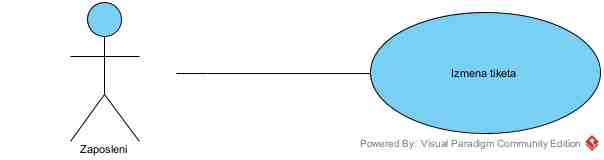
\includegraphics[scale=0.5]{IzmenaTiketa.jpg}



\section{Slučaj upotrebe: Kreiranje zahteva}
\begin{enumerate}
    \item \textbf{Kratak opis:} Zaposleni na osnovu unete opcije i popunjavanja odgovarajucih polja kreira zahtev, koji je nakon kreiranja u statusu nerazrešen.
    \item \textbf{Učesnici:}
        \begin{itemize}
            \item Zaposleni
        \end{itemize}
    \item \textbf{Preduslovi:} Zaposleni je registrovan korisnik sistema.
    \item \textbf{Postuslovi:} Zahtev je uspešno kreiran i sačuvan je u sistemu. Baza je ažurirana i na stranici za prikaz zahteva je dodat novokreirani zahtev
    \item \textbf{Osnovni tok:}
        \begin{enumerate}
            \item Zaposleni otvara stranicu za kreiranje zahteva.
            \item U padajućoj listi bira tip zahteva koji želi da kreira.
            \item Ako je odabrana opcija za rad od kuće, izvršava se podtok (a), ako je odabrana opcija za koriscenje benefita izvršava se podtok (b), ako je izabrana opcija za godišnji odmor izvršava se podtok (c), ako je odabrana opcija za sick leave (d), a ako je odabrana opcija za reevaluaciju izvršava se podtok (e).
            \item Nakon popunjavanja forme, pritiska dugme za potvrdu unosa podataka.
            \item Sistem vrši obradu unosa. Baza je ažurirana. Stranica sa zahtevima je ažurirana.
            \item Na stranici se prikazuje poruka o uspešno kreiranom zahtevu.
        \end{enumerate}
    \item \textbf{Podtokovi:}
        \begin{enumerate}
            \item Rad od kuće
            \begin{enumerate}
                \item Na stranici se prikazuje forma koja sadrži polje za unos datuma kao i polje gde se navodi razlog za zahtev za rad od kuće.
                \item Klikom na polje za unos datuma, zaposlenom se prikazuje padajuci prozor za odabir datuma.
                \item Zaposleni odabira datum.
                \item Zaposleni navodi razlog za podnošenje zahteva. 
            \end{enumerate}
            \item Korišćenje benefita
            \begin{enumerate}
                \item Na stranici se prikazuje padajuća lista sa tipom benefita koji zaposleni želi da odabere.
                \item Zaposleni bira tip benefita.
            \end{enumerate}
            \item Godišnji odmor
            \begin{enumerate}
                \item Na stranici se prikazuje forma koja sadrži dva polja za unos datuma, koja predstavljaju period korišćenja godišnjeg odmora.
                \item Zaposleni preko padajućeg menija bira datum početka i datum kraja korišćenja godišnjeg odmora. 
            \end{enumerate}
            \item Sick leave
            \begin{enumerate}
                \item Na stranici se prikazuje forma koja sadrži dva polja za unos datuma koja predstavljaju period korišćenja godišnjeg odmora, kao i dugme za unos lekarskog izveštaja.
                \item Zaposleni preko padajućeg menija bira datum početka i datum kraja korišćenja sick leave-a.
                \item Zaposleni klikom na dugme unosi dokument koji predstavlja lekarski izveštaj.
            \end{enumerate}
            \item Re-evaluacija
            \begin{enumerate}
                \item Na stranici se prikazuje forma koja sadrži polje gde se unosi razlog za evaluaciju.
            \end{enumerate}
    \end{enumerate}
    \item \textbf{Alternativni tokovi:}
            \begin{enumerate}
                \item Ako je u koraku (iii) podtoka (a) odabran dan koji je u prošlom vremenu(iza trenutnog dana) na ekranu će se prikazati odgovarajuća poruka o grešci. Proces se nastavlja u koraku (iii) podtoka (a).
                \item Ako su u koraku (ii) podtoka (c) odabrani dani sa kojima se premašuje broj dana odmora, na ekranu će se prikazati odgovarajuća poruka o grešci. Proces se nastavlja u koraku (ii) podtoka (c).
                \item Ako su u koraku (ii) podtoka (d) odabrani dani sa kojima se premašuje broj sick leave-a, na ekranu će se prikazati odgovarajuća poruka o grešci. Proces se nastavlja u koraku (ii) podtoka (d). 
            \end{enumerate}
    \item \textbf{Specijalni zahtevi:} /
    \item \textbf{Dodatne informacije:} /
\end{enumerate}

\section{Slučaj upotrebe: Pregled iskorišćenosti dana odmora i sick leave-a}
\begin{enumerate}
    \item \textbf{Kratak opis:} Zaposleni na osnovu odabira tipa odsustva(godišnji odmor ili sick leave) pregleda broj neiskorišćenih dana za odabrani tip odsustva.
    \item \textbf{Učesnici:}
        \begin{itemize}
            \item Zaposleni
        \end{itemize}
    \item \textbf{Preduslovi:} Zaposleni je registrovani korisnik sistema.
    \item \textbf{Postuslovi:} Zaposlenom je prikazan broj neiskorišćenih dana za odabrani tip odsustva, kao i lista iskorišćenih dana odsustva.
    \item \textbf{Osnovni tok:}
        \begin{enumerate}
            \item Zaposleni otvara stranicu za pregled odmora.
            \item U padajućoj listi zaposleni bira da li želi da mu se prikaže broj slobodnih dana odmora ili sick leave-a.
            \item Sistem vrši obradu zahteva.
            \item U zavisnosti od odabranog tipa na ekranu se prikazuje o broju preostalih dana za odabrani tip kao i lista iskorišćenih dana.
        \end{enumerate}
    \item \textbf{Alternativni tokovi:} /
    \item \textbf{Podtokovi:} /
    \item \textbf{Specijalni zahtevi:} /
    \item \textbf{Dodatne informacije:} /
\end{enumerate}


\section{Slučaj upotrebe: Pregled zahteva zaposlenog}
\begin{enumerate}
    \item \textbf{Kratak opis:} Zaposleni na osnovu odabira statusa zahteva(ne razrešen, odobren ili odbijen) pregleda kreirane zahteve od statusa kojeg je odabrao.
    \item \textbf{Učesnici:}
        \begin{itemize}
            \item Zaposleni
        \end{itemize}
    \item \textbf{Preduslovi:} Zaposleni je registrovani korisnik sistema.
    \item \textbf{Postuslovi:} Zaposlenom je prikazana lista zahteva na osnovu statusa kojeg je odabrao.
    \item \textbf{Osnovni tok:}
        \begin{enumerate}
            \item Zaposleni otvara stranicu za pregled zahteva.
            \item U padajućoj listi zaposleni bira status zahteva.
            \item Sistem vrši obradu zahteva.
            \item U zavisnosti od odabranog statusa na ekranu se prikazuje lista zahteva koje je korisnik kreirao.
        \end{enumerate}
    \item \textbf{Alternativni tokovi:} /
    \item \textbf{Podtokovi:} /
    \item \textbf{Specijalni zahtevi:} /
    \item \textbf{Dodatne informacije:} /
\end{enumerate}



\end{document}